\chapter{Исследовательская часть}

\section{Технические характеристики}

Характеристики используемого оборудования:
\begin{itemize}
    \item Микроконтроллер STM32F303 с ОЗУ 48Кб, процессор  до 72 Мгц \cite{bib1}
\end{itemize}

\section{Время выполнения алгоритмов}

В таблице \ref{tbl:time_measurements} приведено время выполнения алгоритмов для разных
квадратных матриц. На рисунке \ref{fig:images-Figure_1} показаны графики
выполнения алгоритмов умножения матриц в миллисекундах (далее --- мс).

\begin{table}[h]
	\begin{center}
		\begin{threeparttable}
		\captionsetup{justification=raggedright,singlelinecheck=off}
		\caption{Время работы алгоритмов (в мс)}
		\label{tbl:time_measurements}
		\begin{tabular}{|c|r|r|r|r|}
			\hline
			Размер матриц &  Классический & Виноград & Виноград оптимизированный \\
			\hline
                        25 & 0.06 & 0.04 & 0.03 \\ \hline 
                        50 & 0.44 & 0.28 & 0.25 \\ \hline 
                        75 & 1.50 & 0.95 & 0.83 \\ \hline 
                        100 & 3.55 & 2.29 & 1.96 \\ \hline 
                        125 & 6.80 & 4.50 & 3.87 \\ \hline 
                        150 & 11.53 & 7.33 & 6.14 \\ \hline 
                        175 & 18.45 & 11.81 & 10.13 \\ \hline 
                        200 & 27.84 & 18.16 & 15.64 \\ \hline 
                        225 & 39.71 & 26.46 & 23.40 \\ \hline 
                        250 & 54.84 & 35.14 & 29.62 \\ \hline 
                        275 & 73.07 & 47.13 & 40.48 \\ \hline 
                        300 & 94.82 & 60.58 & 51.38 \\ \hline 
		\end{tabular}
		\end{threeparttable}
    \end{center}
\end{table}


\clearpage

\begin{figure}[h]
    \centering
    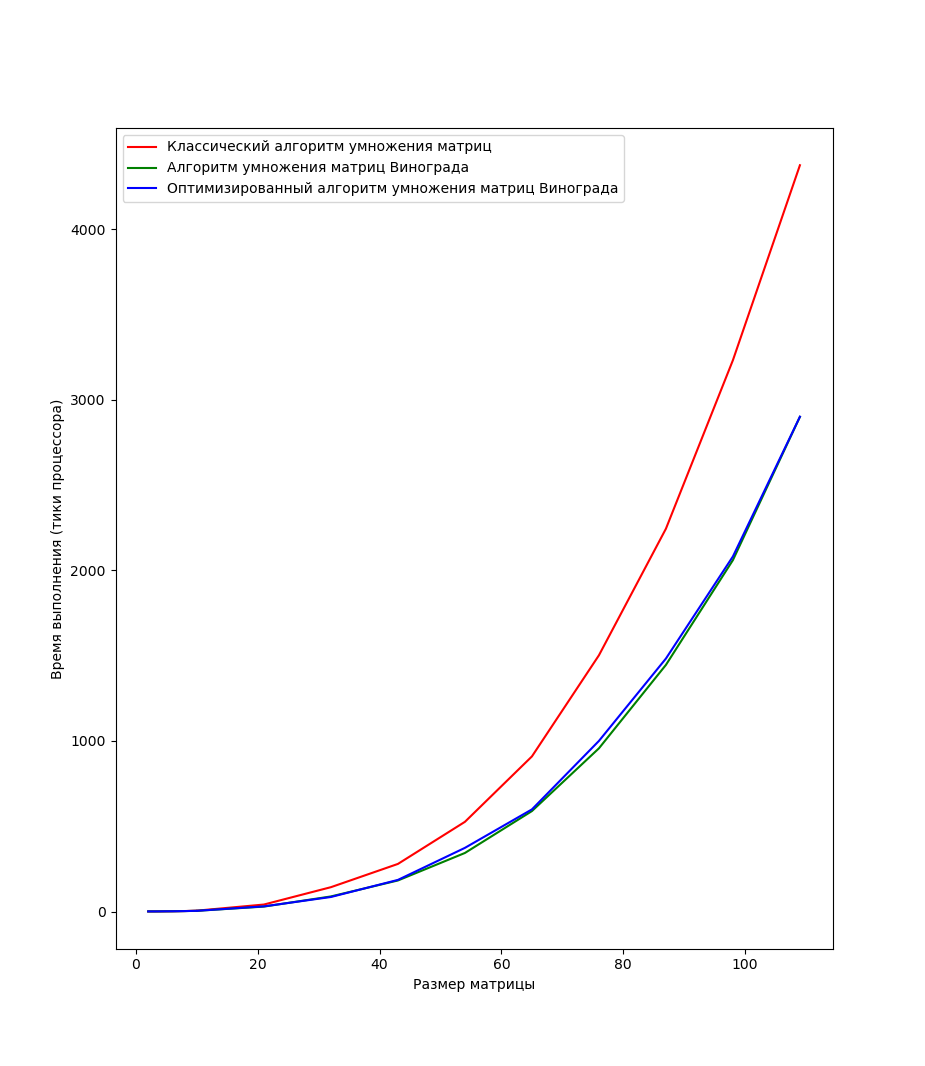
\includegraphics[width=0.8\textwidth]{images/Figure_1}
    \caption{Графики времени выполнения алгоритмов в мс}
    \label{fig:images-Figure_1}
\end{figure}

\section{Вывод}

Сравнения проводились на квадратных матрицах четного и нечетного размера.
Самое долгое время выполнения у алгоритма классического умножения матриц.
Оптимизированный алгоритм Винограда демонстрирует самое быстрое время выполнения.
Неоптимизированный алгоритм Винограда быстрее классического умножения матриц,
но медленнее оптимизированного алгоритма Винограда.

